
\section{Estimating the Central Subspace with Many Environments}
In this section we first provide a naive approach for estimating the central subspace under the invariance assumption \ref{assum:invariance}.
We then elaborate on our proposed method and comment on its differences with the naive approach.

Consider a prior weight vector $w \in \mathbb{R}_{+}^{\abs{\environments}}$ over the environments satisfying $\sum_{e \in \environments} w_e = 1$.
In order to use the information from all environments and all models we aggregate the EGOP matrices using the prior $w$ and define,
$$ M^{w} := \sum_{e,e' \in \environments} \sqrt{w_e} \sqrt{w_{e'}} M^{e,e'} = U^{w} \Lambda^w {V^{w}}^{\T} \in \mathbb{R}^{d \times d}  $$
where the second equality is its singular value decomposition. In the following we establish that this aggreagation provides a feasible estimator for the central subspace.
\begin{proposition}
    \label{prop:weighted-aggregation}
    Under the invariant assumption \ref{assum:invariance} the column space of the weighted aggregated EGOP $M^{w}$ recovers the central subspace, i.e.
    $$ \col\left( M^{w} \right) = \col\left( U^{w} \right) = \mathscr{L} $$
\end{proposition}
The proof is a simple extension of Proposition \ref{prop:identifiability} and we defer it to appendix. 
Although, the choice of prior doesn't explicitly play a role in Proposition \ref{prop:weighted-aggregation}, however, it can be crucial in finite sample estimates.
This is because one expects the convergence rates for EGOP estimates to their population counterparts, i.e. $\hat{M}^{w} \to M^{w}$ when $n_e \to \infty$, to depend on the ill-conditioning of $M^{w}$,
that is how far the $k$'th largest ingular value is from the largest. The optimal choice of prior can remedy this, yet it is unknown to the statistician apriori.
We define our finite-sample naive estimator in the following using a fixed weighting choice. 
\begin{definition}[Naive estimator]
    Suppose $\hat{M}^{e,e'} \subset \mathbb{R}^{d \times d}$ to be EGOP estimates defined in \ref{def:egop-per-env} for a pair of environments $e,e' \in \environments$. 
    Then the naive estimator for central subspace can be obtained from column space of $\hat{M}^w$ with uniform prior $w_e = \frac{1}{T}$,
    $$ \hat{\mathscr{L}}^{\operatorname{naive}} = \col\left( \hat{M}^w \right)$$
\end{definition}

In order to put this estimator into perspective we resort to an optimisation representation of singular value decomposition.
Recall that the $i$'th singular vector of a matrix can be iteratively constructed based on previous singular vectors using the following optimization problem,
\begin{equation*}
    (U_i^w, V_i^w) = \operatorname*{arg\,max}_{ \substack{u,v \in \mathbb{S}^{d} \\ \forall j < i,\, u^{\T} U_j^{w} = 0 \\ \forall j < i,\, v^{\T} V_j^{w} = 0} } u^{\T} M^w v = \sum_{e,e' \in \environments} \sqrt{w_e} u^{\T} M^{e,e'} v \sqrt{w_{e'}}
\end{equation*}
This is in contrast to our approach which solves a more flexible optimization problem with less constraints but tunes the weights,
\begin{equation*}
    (U_i^{\environments}, V_i^{\environments}) = \operatorname*{arg\,max}_{ \substack{u^{e},v^{e} \in \mathbb{S}^{d} \\ \forall j < i,\, \sum_{e \in \environments}  {u^e}^{\T} U_j^{e} = 0 \\ \forall j < i,\, \sum_{e' \in \environments} {v^{e'}}^{\T} V_j^{e'} = 0} } \sum_{e,e' \in \environments} {u^e}^{\T} M^{e,e'} {v^{e'}} 
\end{equation*}
In other words the naive estimator can be thought of as a form of parameter sharing where $u^{e} = \sqrt{w^{e}} u$ and $v^{e} = \sqrt{w^e} v$ for all envrionments $e \in \environments$. This constraint might be benficial in the presence of a shared structure however the advantage of our method is that it also optimally tunes the weights to aggregate different environments.

\begin{figure}[t!]
    \label{fig:results}
    \centering
    \begin{minipage}{0.5\textwidth}
        \centering
        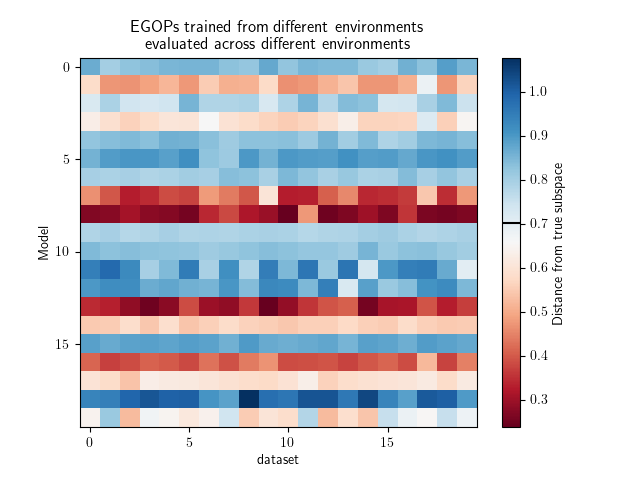
\includegraphics[width=\textwidth]{individual_performance.png}
    \end{minipage}
    \begin{minipage}{0.45\textwidth}
        \centering
        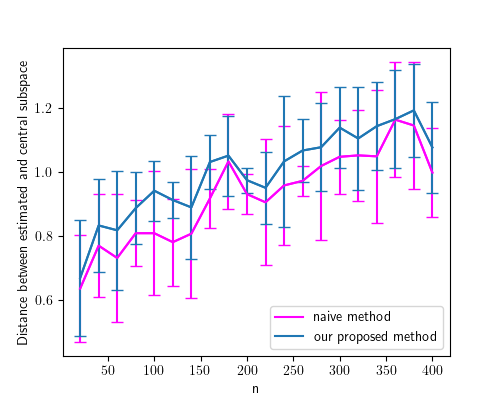
\includegraphics[width=\textwidth]{final_res.png}
    \end{minipage}
    \caption{(left) The performance of subspace estimates $\hat{\mathscr{L}}^{e,e'}$ based on individual EGOPs $\hat{M}^{e,e'}$. Rows represent the model index and columns represent the dataset which is evaluated on. 
    (right) The performance of our method on average dominates the naive method performance.}
\end{figure}

